\documentclass{article}
\title{Blanchard Ch.10}
\author{Dawei Wang}
\date{\today}
\usepackage{ctex}
\usepackage{amsmath}
\usepackage{amssymb}
\usepackage{graphicx} %插入图片的宏包
\usepackage{float} %设置图片浮动位置的宏包
\usepackage{subfigure} %插入多图时用子图显示的宏包
\begin{document}
	\maketitle
\section{生活水准(standard of living)的衡量}

人均产出(output per person/out put per capita),假定产出和收入相等,则人均产出就是人均收入。

\hspace*{\fill}

以汇率计算人均产出的缺点:

汇率波动大;

通货膨胀,一般来说,一个国家的人均产出越低,该国家的食品和基本生活服务的价格也越低。

购买力平价(purchasing power parity,PPP)修正了汇率的波动以及国家间价格的系统性区别的影响来比较两个国家的生活水准

\hspace*{\fill}

人们的福利水平是由他们的消费,而不是收入决定的。因此可以用人均消费而不是人均产出水平来衡量生活水准。

从生产的角度看,有人可能会对国家间的生产率差异而不是生活水准差异感兴趣,在这种情况下,合适的度量指标应该是单位工人的平均产量,或者更恰当的每工时产量,而不是人均产出。

生活水平高幸福程度就一定高吗?钱会带来幸福。

\subsection{解读购买力平价}

两个国家用一样的价格分别去衡量每个国家能消费每种商品的数量。这种计算方法,用同样的一系列价格度量不同国家的变量,就是购买力平价理论的度量方法。购买力平价用的是国家间的平均价格,称为国际美元价格。

\subsection{钱能带来幸福吗}

一旦基本需求得到满足,人均收入的增加就不会增加幸福感;重要的不是绝对收入水平,而是相对收入水平。

虽然个人的幸福肯定不仅取决于收入,但它肯定会随着收入增加。不过收入水平超过某个关键水平后就不再对幸福水平产生直接影响。经济中的许多其他方面对福利很重要,收入分配肯定是其中之一。

\section{考察增长:入门知识}

\subsection{总量生产函数}

总量生产函数(aggregate production function)代表总产出与投入的一种特定关系。

如果我们只关注产出和就业的波动,那么$ Y=N $这个线性关系就是成立的。但我们现在转向研究经济增长,假设工人的人均产出是恒定的,即不考虑人均产出的增长就是不切实际的了。现在放松假定条件,假定有两种投入要素——资本和劳动力,则产出和投入的关系式为:

\[
Y=F(K,N)
\]

这种研究产出的方式没有区分不同资本品之间的作用的差别,也没有对劳动力进行区分。重点在于强调了资本和劳动力都对总产出有影响。

技术状态(state of technology)描述了给定数量的劳动力和资本能有多少产出,即将产出和两种投入要素联系起来,表现了总量生产函数的具体形式。

\subsection{规模报酬和要素报酬}

规模报酬不变:

\[
xY=F(xK,xN)\enspace for\enspace all\enspace x\in R_+
\]

增加投入要素,产出肯定增加。但固定其中一种投入,另外一种投入增加导致的产出增加将越来越少,这就叫投入要素(资本/劳动力)的规模报酬递减。

\subsection{人均产出和人均资本}

假设规模报酬不变,结合生产函数,我们可以得到人均产出和人均资本的关系式:

\[
\frac{Y}{N}=F(\frac{K}{N},\frac{N}{N})=F(\frac{K}{N},1)
\]

$ Y/N $是人均产出,$ K/N $是人均资本,上式说明人均产出决定人均资本量。

\begin{figure}[H] %H为当前位置,!htb为忽略美学标准,htbp为浮动图形
	\centering %图片居中
	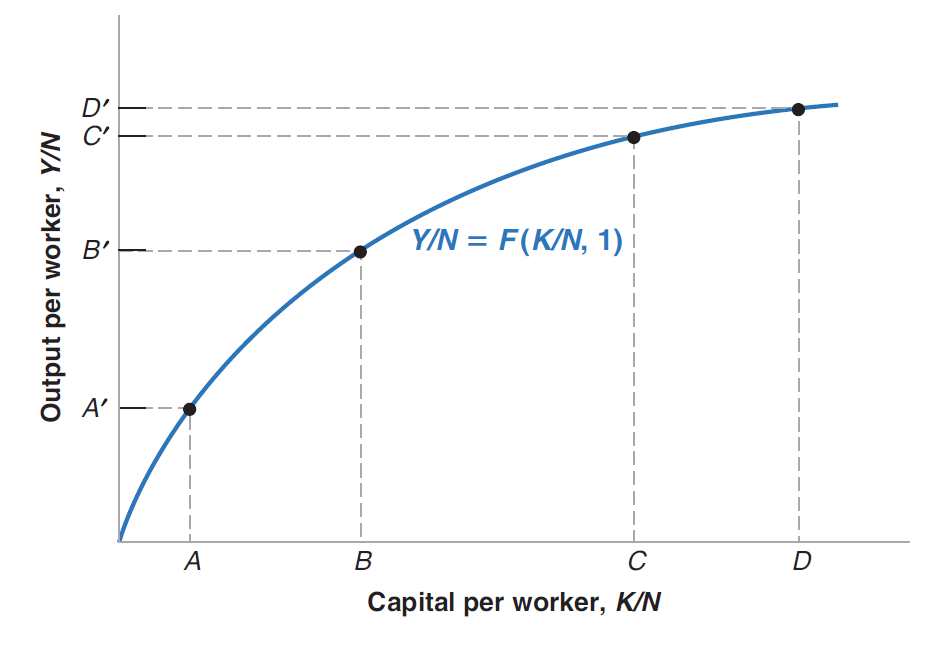
\includegraphics[width=1\textwidth]{10_1} %插入图片,[]中设置图片大小,{}中是图片文件名
	\caption{Output and Capital per
		Worker} %最终文档中希望显示的图片标题
	\label{Fig.main2} %用于文内引用的标签
\end{figure}

曲线向上倾斜表示随着人均资本增加,人均产出相应增加。曲线向上凸表示随着资本增加,产出增加的幅度会越来越小,这符合资本的规模报酬递减。

\subsection{增长的源泉}

假设劳动者占人口的比例保持不变,为什么人均产出会随着时间增长?

人均产出$ Y/N $的增加可能来自人均资本$ K/N $的增加:当$ K/N $增加,沿着横轴向右边移动,$ Y/N $增加。

人均产出增加也可能来源于技术进步。人均资本量给定,技术进步导致生产函数F移动,人均产出增加。

\begin{figure}[H] %H为当前位置,!htb为忽略美学标准,htbp为浮动图形
	\centering %图片居中
	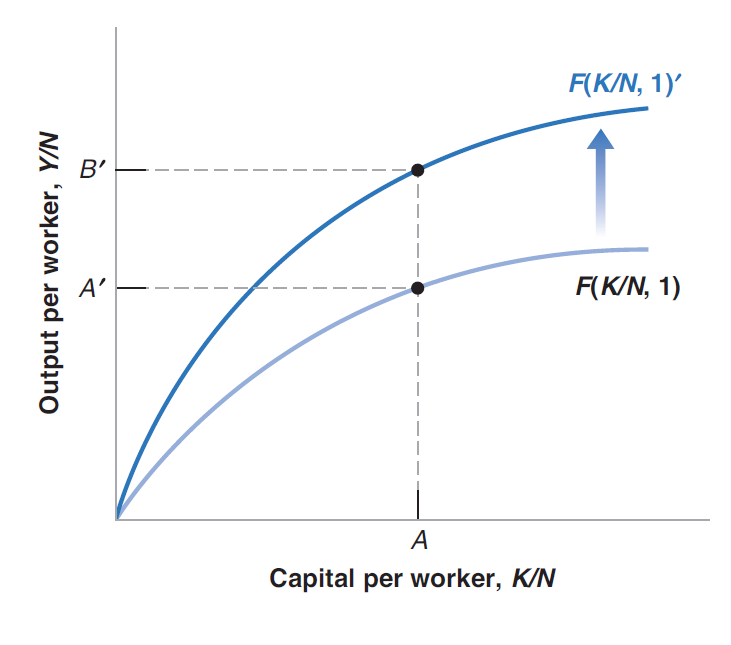
\includegraphics[width=1\textwidth]{10_2} %插入图片,[]中设置图片大小,{}中是图片文件名
	\caption{The Effects of an
		Improvement in the State
		of Technology} %最终文档中希望显示的图片标题
	\label{Fig.main3} %用于文内引用的标签
\end{figure}

因此,我们可以认为经济增长源于资本积累(capital accumulation)和技术进步(technological progress),然而,这两个因素在增长过程中的作用完全不同。

资本积累本身并不能维持稳定增长。由于资本的规模报酬递减,保持人均产出的稳定增长需要投入越来越多的人均资本。在某一阶段,经济不会或者不能储蓄进而投资更多的资本,这时人均产出会停止增长。

这意味着一个经济体的储蓄率(saving rate,储蓄占收入的比例)也很重要,储蓄虽然不能一直提高增长水平,但是较高的储蓄率能带来较高的产出水平。

\hspace*{\fill}

持续的技术进步才能带来持续的增长。人均产出的增长率最终取决于技术进步的速度,这意味着一个经济体能保持技术进步较快,则其最终会赶超其他经济体。

\hspace*{\fill}

技术发展水平的两个定义:

狭义的定义是当前经济体中可用的技术;

广义的定义是经济体的组织方式,从制度本身到政府效率等。







	
\end{document}